%%%%%%%%%%%%%%%%%%%%%%%%%%%%%%%%%%%%%%%%%%%%%%%%%%%%%%%%%%%%%%%%%%%%%%%%
\chapter{Implementación}
\label{ch:implemetacion}
 En este capítulo se describirán todos los detalles relativos a la implementación de la aplicación. Empezaremos detallando el entorno de ejecución y el lenguaje de programación usado para su desarrollo y terminaremos destacando los detalles relevantes de la implementación. A saber:
 
\section{Entorno de ejecución}
 La aplicación desarrollada se ejecuta en un entorno llamado \emph{Cocoa Touch}. Cocoa es un conjunto de frameworks orientados a objetos que proporcionan un entorno de ejecución para las aplicaciones que se ejecutan en el sistema operativo \emph{iOS}. Este entorno de desarrollo nos facilita a los desarrolladores la tarea de pasar de la etapa de diseño a la etapa de desarrollo para crear una aplicación. \emph{Cocoa Touch} proviene del entorno de la plataforma \emph{Mac OS}, entorno de los que dependen los equipos de sobremesa de Apple. Se puede decir que es la misma plataforma añadiendo el soporte para los eventos táctiles y orientados a la tecnología móvil. 
 
 \emph{Cocoa} presenta dos caras: 
 \begin{itemize}
	\item Entorno de ejecución: las aplicaciones desarrolladas en Cocoa presentan la interfaz de usuario de la aplicación y están fuertemente integradas con otras partes del sistema operativo como por ejemplo el buscador del sistema de ficheros.
	\item Entorno de desarrollo: Cocoa es una suite de componentes software que están orientados a objetos y que te permiten rápidamente crear robustas y completas aplicaciones para el sistema operativo.
\end{itemize}
  
 \begin{figure}[ht!]
    \centering
       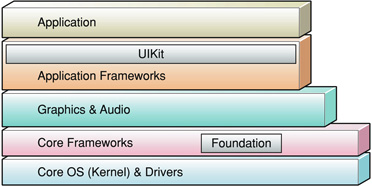
\includegraphics[width=0.9\textwidth]{./images/architecture_stack.jpg}
     \caption{Entorno \emph{iOS}}
   \label{fig:iOS Platform}
\end{figure}
 
 A pesar de que la estructura del \emph{iOS} es similar a la de la plataforma \emph{Mac OS}, existen diferencias significantes. El diagrama del \emph{iOS} muestra una plataforma como una serie de capas que van desde en núcleo de sistema operativo hasta un conjunto de frameworks de aplicación, la más crítica (para las aplicaciones) empieza con la capa UIKit.
 
 Para desarrollar en entornos \emph{Cocoa} se utiliza el lenguaje \emph{Objective-C}. Este lenguaje está basado en la programación orientada a objetos. Se define como un superconjunto del lenguaje de programación \emph{C}, es decir, podemos considerarle como una fina capa que complementa a \emph{C}. La sintaxis de objetos de \emph{Objective-C} deriva de \emph{Smalltalk}\footnote{Smalltalk es un lenguaje de programación que permite realizar tareas de computación mediante la interacción con un entorno de objetos virtuales.}.
 
  Como todo lenguaje de programación orientado a objetos, \emph{Objective-C} nos proporciona principalmente:
 \begin{itemize}
	\item Un lenguaje de programación orientado a objetos.
	\item Una extensa librería de objetos.
	\item Una conjunto software de herramientas de desarrollo.
	\item Un entorno de ejecución propio.
\end{itemize}

 Aparte de las características propias del lenguaje, al estar basado en el lenguaje \emph{C}, su compilador es capaz de ejecutar líneas de código codificadas en \emph{C}. Esta característica permite usar librerías realizadas en \emph{C} en programas desarrollados en \emph{Objective-C}.  En el presente trabajo hemos optado por usar el lenguaje \emph{Objective-C} en todo el desarrollo por ser el recomendado por Apple para una mejor integración con \emph{iOS}.
 
\section{Estructura de la aplicación}
 Cuando construimos una aplicación para el sistema operativo \emph{iOS} usamos la herramienta que nos proporciona el SDK de Apple \emph{Xcode}. Es un editor software que contiene todos lo necesario para compilar proyecto escrito en \emph{Objective-C}. La ventaja de usar este editor y no uno universal que acepte dicho lenguaje de programación es que \emph{Xcode} es capaz de implementar nuestra aplicación en lo que llamamos un paquete. Este paquete es un directorio en el sistema de ficheros que agrupa los recursos necesarios para la aplicación en un mismo lugar. Dicho paquete contiene el ejecutable y cualquier recurso usado por el mismo (por ejemplo, el icono de la aplicación, imágenes contenidas \ldots). El siguiente cuadro lista el contenido del paquete de esta aplicación.
 
\begin{center}
\tablefirsthead{\hline\hline\rowcolor[gray]{0.9}Archivo & Descripción\\\hline\hline}
\tablehead{\hline\hline\rowcolor[gray]{0.9}Archivo & Descripción\\\hline\hline}
% \tabletail{}
% \tablelasttail{}
\bottomcaption{Contenido de un paquete Xcode Cap}
\begin{supertabular}{||p{0.45\linewidth}|p{0.45\linewidth}||}
\lstinline!BetfairApp! & El fichero ejecutable de la aplicación. El nombre de este fichero es el mismo que el de la aplicación más la extensión app.\\ 
\hline 
\lstinline!Default.png! & Imagen de 480 x 320 píxeles que se muestra nada más iniciarse la aplicación  a modo de introducción. El sistema usa esta imagen mientras realiza tareas en segundo plano que requieren de un tiempo sensible para el usuario.\\
\hline
\lstinline!Settings.bundle! & Es un fichero que contiene las preferencias de la aplicación a personalizar por el usuario, como por ejemplo el lenguaje de la aplicación, el tipo de moneda a mostrar\ldots \\
\hline
\lstinline!iconBF.png! & Icono de 57 x 57 píxeles que representa la aplicación en la pantalla principal del dispositivo. \\
\hline
\lstinline!Info.plist! & También conocida como lista de propiedades. Este fichero es un lista donde se definen los valores claves de la aplicación tales como el identificador de aplicación, la versión y el título.\\
\hline
\lstinline!en.lproj! & Archivo que contiene los textos de la interfaz en inglés. Usado por el sistema cuando este lenguaje esta por defecto para lanzar aplicación o definido en las preferencias de la aplicación.\\
\hline
\lstinline!es.lproj! &Archivo que contiene los textos de la interfaz en español.\\
\hline
\lstinline!MainWindows.xib! & Contiene la interfaz a cargar por defecto por el sistema una vez lanzada la aplicación. Contiene la ventana principal de la interfaz de usuario. \\
\hline
\lstinline!RootViewController.xib! & Contiene los objetos necesarios de la interfaz de usuario del menú principal. \\
\hline
\lstinline!EventsControllerView.xib! &Contiene los objetos necesarios de la interfaz de usuario del menú de los eventos activos. \\
\hline
\lstinline!EventsTypesControllerView.xib! & Contiene los objetos necesarios de la interfaz de usuario de los tipos de eventos de Betfair. \\
\hline
\lstinline!EventsAndMarketsControllerView.xib! & Contiene los objetos necesarios de la interfaz de usuario de los eventos y mercados disponibles. \\
\hline
\lstinline!MarketInfoControllerView.xib! & Contiene los objetos necesarios de la interfaz de usuario de las características de un mercado. \\
\hline
\lstinline!PutBetControllerView.xib! & Contiene los objetos necesarios de la interfaz de usuario de la realización de una apuesta. \\
\hline
\lstinline!MyBetsControllerView.xib! & Contiene los objetos necesarios de la interfaz de usuario del menú de las apuestas ya realizadas por el usuario. \\
\hline
\lstinline!MyBetsCategoryController.xib! & Contiene los objetos necesarios de la interfaz de usuario de las categorías de apuestas realizadas por el usuario. \\
\hline
\lstinline!MyBetsDetailsView.xib! & Contiene los objetos necesarios de la interfaz de usuario con los detalles de una apuesta ya realizada y las opciones disponibles. \\
\hline
\lstinline!MyBetPropertiesView.xib! & Contiene los objetos necesarios de la interfaz de usuarios de los datos del mercados en los que se realizó la apuesta con las opciones posibles a realizar sobre esta. \\
\hline
\lstinline!TradingController.xib! & Contiene los objetos necesarios de la interfaz de usuario con los detalles acerca del trading sobre una apuesta. \\
\hline 
\hline 
\end{supertabular} 
\label{fig:componentes}
\end{center} 

\section{Internacionalización}
 Una parte importante a destacar en el proyecto es la posibilidad de establecer el idioma de la aplicación. Mediante la tienda de aplicaciones \emph{iTunes App Store} se puede distribuir la aplicación por diferentes países. Una aplicación de \emph{iOS} debe tener la posibilidad de poder mostrar varios idiomas y tener uno por defecto. Cada lenguaje esta implementado en la carpeta \emph{nombre-aplicación.lprj} del paquete de implementación ya comentado en el cuadro \ref{fig:componentes}. En el conjunto para proporcionar el soporte a distintos idiomas también se podrá especificar una imagen de portada, icono de la aplicación, mensajes de alerta\ldots  adecuado al idioma escogido por el usuario. Por defecto, el sistema operativo \emph{iOS} arranca la aplicación con los argumentos necesarios para que muestre la aplicación en el mismo idioma especificado en las preferencias del terminal, es decir, es el mismo lenguaje que esté configurado en éste. En caso de que no fuera posible, se procederá con el especificado por defecto de la aplicación.

  \begin{figure}[h!]
    \centering
       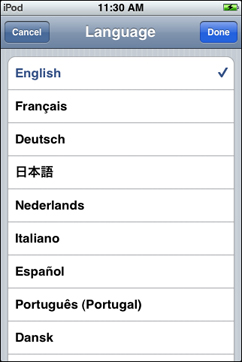
\includegraphics[width=0.5\textwidth]{./images/language.jpg}
     \caption{Ejemplo de la elección del idioma }
   \label{fig:Vista de las preferencias del idioma}
\end{figure}

 
  En esta implementación se procederá a dar soporte al español y al inglés, dos de los lenguajes más hablados dentro de la lista mundial.
  
  
  
  \begin{figure}[h!]
  	\centering 
  		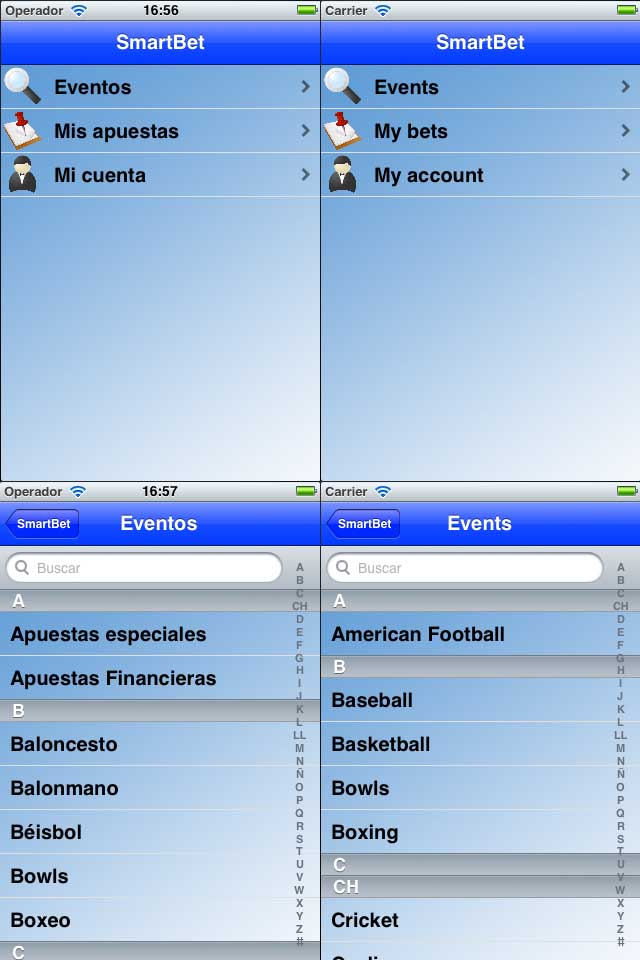
\includegraphics[width=0.7\textwidth]{./images/lenguajes.jpg}
	\caption{Ejemplo de interfaz con distinto idioma seleccionado.} 
	\label{fig:Ejemplo de interfaz con distinto idioma seleccionado.}
\end{figure} 
  
  
  
  Para implementar esta funcionalidad dentro de nuestro trabajo de fin de carrera hemos de definir la lista de palabras a traducir dentro de un archivo llamado \emph{Localizable.strings}.  Este archivo contiene una lista de la tupla etiqueta-traducción. El sistema, cada vez que encuentra una etiqueta en la interfaz de usuario la sustituye por la traducción del idioma en el que este configurado el terminal. A continuación se muestra un ejemplo del contenido de dicho fichero.
  
\begin{lstlisting}
/* 
   Localizable.strings
   Betfair App

   Created by Francisco on 21/12/11.
   Copyright 2011  . All rights reserved.
*/
"Events" = "Eventos";
"My bets" = "Mis apuestas";
"My account" = "Mi cuenta";
"Announcements" = "Mensajes del sistema";
"Profile" = "Cuenta";
"Bet info" = "Info. apuesta";
"Your bet" = "Tu apuesta";
"Nothing" = "Vacio";
"Active events" = "Eventos activos";
"Available markets" = "Mercados disponibles";
"Bet for" = "Apostar por";  
\end{lstlisting}

  
   Por ejemplo, para mostrar el título ``Mis Apuestas'' en español el sistema buscará la etiqueta en el archivo \emph{Localizable.string} perteneciente al idioma español. En el código especificaremos la etiqueta a mostrar ``My bets'' y el sistema, en tiempo de ejecución, mostrará su traducción, en este caso ``Mis apuestas''.  Este archivo se ubica dentro de la carpeta es.lpjr o en.lpjr según sea la tabla de traducción en inglés o en español. 
   
   Berfair, en su \emph{API} nos permite especificar en cada servicio en que idioma queremos recibir la respuesta. Con la combinación de ambas funcionalidades tenemos en el presente fin de carrera la aplicación completamente traducidas en dos idiomas disponibles: inglés y español. 
   
\section{Interpretación XML de Betfair a Cocoa Touch}
 Como ya tratamos en el capítulo \ref{ch:diseno}, un tema clave a destacar es la adaptación del \emph{API} de Betfair a la arquitectura del terminal iPhone. 
 
  Betfair ofrece el acceso a todos sus servicios a aquellos programadores que quieren incluirlos a través de aplicaciones. Es un camino eficaz para hacer llegar sus servicios a usuarios de otras plataformas o para usuarios expertos que requieran de una interfaz de usuario más experta, orientada a sus necesidades. Por supuesto que esta política requiere de un sistema de seguridad para evitar fraudes o ataque por parte de la comunidad de hackers.
   
  En el diseño de una aplicación que debe hacer uso de servicios web ofrecidos por un sistema externo se necesita algún tipo de \emph{API} o interfaz para acceder a los mismos. Lo primero a tener en cuenta es lo que se necesita para hacer uso de las funciones proporcionadas por el \emph{API}. Para acceder a los servicios ofrecidos por Betfair, como ya vimos en la figura \ref{fig:servicioweb} necesitamos conocer la interfaz de acceso que se describe  en un archivo en formato WSDL. Este tipo de archivo es muy común y se usa para describir interfaces públicas de acceso a servicios web. Está basado en XML y contiene los requisitos, parámetros y formatos de los mensajes necesarios para interactuar con los servicios disponibles. 
   
   Existen herramientas en el mercado que traducen de forma automática el archivo WSDL en código fuente ahorrando al programador tiempo y excluyendo al mismo los aspectos más básicos de la comunicación. Siendo \emph{iOS} una plataforma novedosa, no existe a día de hoy este tipo de herramientas por lo que se tuvo que afrontar el desarrollo de la comunicación con el servidor de Betfair.
      
   A continuación se muestra un fragmento del archivo WSDL de Betfair. En este caso describe los parámetros necesarios para hacer uso del servicio \emph{Login } (\lstinline{Login}).
   
\begin{lstlisting}[language=xml]
<xsd:complexType name="LoginReq">
 <xsd:sequence>
  <xsd:element name="ipAddress" nillable="false" type="xsd:string"/>
  <xsd:element name="locationId" nillable="false" type="xsd:int"/>
  <xsd:element name="password" nillable="false" type="xsd:string"/>
  <xsd:element name="productId" nillable="false" type="xsd:int"/>
  <xsd:element name="username" nillable="false" type="xsd:string"/>
  <xsd:element name="vendorSoftwareId" nillable="false" type="xsd:int"/>
 </xsd:sequence>
</xsd:complexType>
\end{lstlisting}

   En el listado podemos comprobar como nos hacen falta 6 parámetros para poder hacer uso del servicio \emph{Login}: \emph{ipAddress}, \emph{locationId}, \emph{password}, \emph{productId}, \emph{username} y \emph{vendorSoftwareId}. Todos estos parámetros nos lo proporciona Betfair cuando nos damos de alta en su programa de desarrollo.
   
   En la aplicación, para comenzar la comunicación con el servidor de Betfair, necesitamos construir la estructura de los mensajes a enviar en formato XML. Para ello, se desglosa el archivo en varias partes. La primera establecer la dirección web donde enviar los mensajes. La segunda construir las estructuras XML de cada servicio web tal y como viene descrito en el archivo WSDL. Hay que recalcar que a cada servicio, lo normal, es tener dos mensajes. El primero donde hacemos la petición al servidor y el segundo la respuesta. Para el caso concreto del \emph{Login} el formato del mensaje en XML a enviar sería el siguiente:
 
\begin{lstlisting}[language=xml]
  <?xml version="1.0" encoding="UTF-8"?>
  <SOAP-ENV:Envelope xmlns:SOAP-ENV="http://schemas.xmlsoap.org/soap/envelope/" xmlns:SOAP-ENC="http://schemas.xmlsoap.org/soap/encoding/" xmlns:xsi="http://www.w3.org/2001/XMLSchema-instance" xmlns:xsd="http://www.w3.org/2001/XMLSchema" xmlns:ns2="http://www.betfair.com/publicapi/types/global/v3/" xmlns:ns1="http://www.betfair.com/publicapi/v3/BFGlobalService/">
  <SOAP-ENV:Body>
  <ns1:login>
  <ns1:request>
  <ipAddress>0.0.0.0</ipAddress>
  <locationId>0</locationId>
  <password>xxxxxxxx</password>
  <productId>82</productId>
  <username>user</username>
  <vendorSoftwareId>0</vendorSoftwareId>
  </ns1:request></ns1:login>
  </SOAP-ENV:Body>
  </SOAP-ENV:Envelope> 
 \end{lstlisting}
 
  Una vez construido el cuerpo del mensaje, sólo nos hace falta conocer la dirección de destino para el mensaje a enviar a los servidores de Betfair. Dicha dirección también viene descrita en el archivo WSDL:
  
\begin{lstlisting}
URL = "https://api.betfair.com/betex-api-public-ws/BFService";
\end{lstlisting}

  Una vez la aplicación ha realizado estos pasos, toda la información se envía a Betfair en un mensaje HTML. 
  
  Una vez enviado el mensaje de petición la aplicación espera la respuesta de Betfair. El formato de la respuesta también viene definido en el archivo WSDL. En este caso la repuesta se recibe con el siguiente formato:

\begin{lstlisting}[language=xml] 
<?xml version="1.0" encoding="UTF-8"?>
<soap:Envelope xmlns:soap="http://schemas.xmlsoap.org/soap/envelope/" xmlns:xsi="http://www.w3.org/2001/XMLSchema-instance" xmlns:n2="http://www.betfair.com/publicapi/types/" xmlns:xsd="http://www.w3.org/2001/XMLSchema">
<soap:Body>
<n:loginResponse xmlns:n="http://www.betfair.com/publicapi/BFService/">
<n:Result xsi:type="n2:LoginResp">
<header xsi:type="n2:APIResponseHeader">
<errorCode xsi:type="n2:APIErrorEnum">OK</errorCode>
<minorErrorCode xsi:nil="1"></minorErrorCode>
<sessionToken xsi:type="xsd:string">6XbAFn0tqfGgdWtQhRmspO</sessionToken>
<timestamp xsi:type="xsd:dateTime">2009-11-23T11:39:45.644Z</timestamp>
</header>
<currency xsi:type="xsd:string">EUR</currency>
<errorCode xsi:type="n2:LoginErrorEnum">OK</errorCode>
<minorErrorCode xsi:nil="1"></minorErrorCode>
<validUntil xsi:type="xsd:dateTime">0001-01-01T00:00:00.000Z</validUntil>
</n:Result>
</n:loginResponse>
</soap:Body>
</soap:Envelope>
 \end{lstlisting}
 
  Lo primera que realiza la aplicación al recibir el mensaje es observar los campos \emph{errorCode}. Este campo nos indica si hay algún problema en los parámetros de la petición anteriormente enviada. En el ejemplo, en ambos casos recibimos un \emph{OK}. Una vez comprobado la coherencia en la respuesta a salvo de fallos de recepción se procede a descifrar la respuesta. Para ello, en la aplicación se implementó un parser que convierte este mensaje en una estructura de datos válida para nuestro desarrollo.  La aplicación procesa el mensaje en XML y finalmente muestra al usuario la información recibida en un formato más adecuado. En la figura \ref{fig:proceso} se muestra el procedimiento completo del proceso.
       
 \begin{figure}[h!]
    \centering
       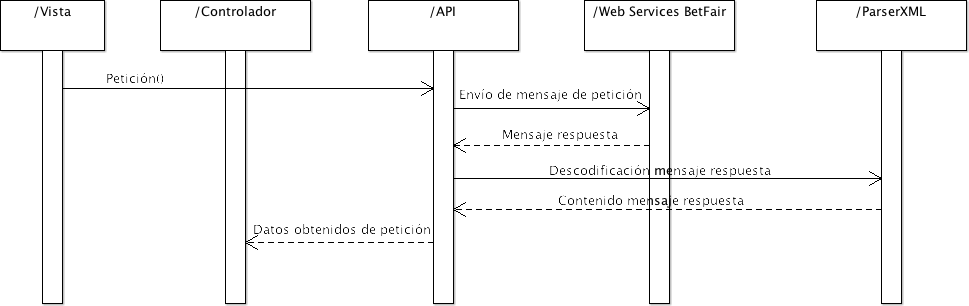
\includegraphics[width=1.2\textwidth]{./images/modelo_accion.png}
     \caption{Ejemplo de comunicación API }
   \label{fig:proceso}
\end{figure}
 
    
    Toda la aplicación gira en torno a este proceso. Sin él es incomprensible el resto del aplicativo. Es en él donde obtenemos los datos directamente de BetFair. Es lógico tratarlo así ya que las aplicaciones móviles suelen usar siempre servicios web y por tanto necesitan de conectividad. Esta aplicación no guarda información alguna salvo las credenciales de acceso al servicio. En una aplicación móvil nos interesa que la información que se necesita esté disponible cualquiera que sea el lugar donde nos encontremos. En el contexto de las apuestas lo más importante es tener la información lo más actualizada posible, es por eso que no se guarda la información de los mercados. Eso sí, tendría sentido quizá dotar en un futuro a la aplicación de una caché ,opcional a la elección del usuario, con caducidad para, por ejemplo, minimizar el consumo de batería del dispositivo en el caso que se necesitase.  
   
%%% Local Variables: 
%%% mode: latex
%%% TeX-master: "tfc-betfair-ios"
%%% TeX-PDF-mode: t
%%% ispell-local-dictionary: "castellano"
%%% End: 
